\documentclass[12pt,a4paper]{report}
% Layout shared by the coursework reports in this repository.
\usepackage{fontspec}
\IfFontExistsTF{DejaVu Sans Mono}{\setmonofont[Scale=0.84]{DejaVu Sans Mono}}{}
\usepackage[vietnamese]{babel}
\usepackage[a4paper,margin=1in]{geometry}
\usepackage{amsmath,amssymb,mathtools,bm}
\usepackage{booktabs,tabularx,array,longtable}
\usepackage{graphicx,float}
\usepackage{enumitem}
\usepackage{fancyhdr,setspace,titlesec,caption,microtype,needspace,etoolbox}
\usepackage[hidelinks]{hyperref}

\setstretch{1.15}
\setlength{\parskip}{0.45em}
\setlength{\parindent}{0pt}
\setlength{\headheight}{16pt}
\setcounter{tocdepth}{2}
\setcounter{secnumdepth}{3}
\emergencystretch=2em

\captionsetup{font=small,labelfont=bf}
\numberwithin{equation}{chapter}

\titleformat{\chapter}[display]
  {\normalfont\bfseries}
  {\filleft\Large\chaptertitlename\ \thechapter}
  {0.35em}
  {\filright\huge}
  [\vspace{0.4em}\titlerule]
\titlespacing*{\chapter}{0pt}{-10pt}{22pt}
\titleformat{\section}{\Large\bfseries}{\thesection}{0.6em}{}
\titleformat{\subsection}{\large\bfseries}{\thesubsection}{0.6em}{}
\titleformat{\subsubsection}{\normalsize\bfseries}{\thesubsubsection}{0.6em}{}

\preto\section{\Needspace{5\baselineskip}}{}
\preto\subsection{\Needspace{4\baselineskip}}{}
\preto\subsubsection{\Needspace{3\baselineskip}}{}

\newcommand{\CourseReportHeader}[1]{%
  \pagestyle{fancy}%
  \fancyhf{}%
  \fancyhead[L]{\small\nouppercase{\leftmark}}%
  \fancyhead[R]{\small #1}%
  \fancyfoot[C]{\thepage}%
  \fancypagestyle{plain}{%
    \fancyhf{}%
    \fancyhead[L]{\small\nouppercase{\leftmark}}%
    \fancyhead[R]{\small #1}%
    \fancyfoot[C]{\thepage}%
  }%
}

\newcommand{\R}{\mathbb{R}}
\newcommand{\norm}[1]{\left\lVert #1 \right\rVert}
\newcommand{\code}[1]{\texttt{\detokenize{#1}}}

% Arguments: logo, report type, course, title, author label, metadata rows, date.
\newcommand{\CourseCover}[7]{%
  \hypersetup{pageanchor=false}%
  \begin{titlepage}
    \centering
    \vspace*{0.5cm}
    {\normalsize\bfseries ĐẠI HỌC QUỐC GIA THÀNH PHỐ HỒ CHÍ MINH\par}
    {\normalsize\bfseries TRƯỜNG ĐẠI HỌC BÁCH KHOA\par}
    {\normalsize\bfseries KHOA KHOA HỌC VÀ KỸ THUẬT MÁY TÍNH\par}
    \vspace{0.6cm}
    \includegraphics[width=0.2\textwidth]{#1}\par
    \vspace{0.7cm}
    {\large\bfseries #2\par}
    \vspace{0.35cm}
    {\normalsize\textbf{#3}\par}
    {\small Học kỳ 261 · Năm học 2026–2027\par}
    \vspace{0.45cm}
    {\LARGE\bfseries #4\par}
    \vspace{0.6cm}
    {\normalsize\bfseries #5\par}
    \vspace{0.35cm}
    {\small\begin{tabular}{@{}ll@{}}#6\end{tabular}\par}
    \vfill
    {\small\bfseries Thành phố Hồ Chí Minh, #7\par}
  \end{titlepage}
  \pagenumbering{roman}%
  \hypersetup{pageanchor=true}%
}

\newcommand{\CourseFrontChapter}[1]{%
  \chapter*{#1}%
  \addcontentsline{toc}{chapter}{#1}%
  \markboth{#1}{#1}%
}

\newcommand{\CourseAbstract}[1]{%
  \CourseFrontChapter{Tóm tắt}%
  #1\par
}

\newcommand{\CourseOverview}[1]{%
  \CourseFrontChapter{Tổng quan báo cáo}%
  \begingroup
  \renewcommand{\arraystretch}{1.3}%
  \begin{tabularx}{\textwidth}{@{}>{\bfseries\raggedright\arraybackslash}p{3.3cm}>{\raggedright\arraybackslash}X@{}}
    #1
  \end{tabularx}
  \endgroup
}

% Omit the figure list for a report containing only tables.
\newcommand{\CourseContents}[1][\listoffigures]{%
  \tableofcontents
  #1%
  \listoftables
  \clearpage
  \pagenumbering{arabic}%
}

\usepackage{tikz}
\usetikzlibrary{arrows.meta}
% Original diagrams matching the E1, E2 and E3 notebook architectures.
% Tensor shapes omit the batch dimension unless stated otherwise.
\tikzset{
  exblock/.style={draw, rectangle, align=center, minimum height=10mm,
    text width=25mm, inner sep=3pt, font=\small},
  extensor/.style={exblock, double, double distance=1pt},
  exarrow/.style={-{Latex[length=2mm]}, semithick},
  exnote/.style={font=\small, align=center},
  exsum/.style={draw, circle, inner sep=1pt, minimum size=6mm, font=\small}
}

\newcommand{\ExerciseOneArchitecture}{%
\begin{figure}[htbp]
\centering
\begin{tikzpicture}[x=1cm,y=1cm]
  \node[exnote,anchor=west] at (-1.4,0.85) {\textbf{Softmax classifier}};
  \node[extensor] (s0) at (0,0) {Image\\$1\times28\times28$};
  \node[exblock] (s1) at (3.1,0) {Flatten\\$784$};
  \node[exblock] (s2) at (6.2,0) {Linear\\$784\to10$};
  \node[extensor] (s3) at (9.3,0) {Logits\\$10$};
  \draw[exarrow] (s0)--(s1); \draw[exarrow] (s1)--(s2); \draw[exarrow] (s2)--(s3);

  \node[exnote,anchor=west] at (-1.4,-1.15) {\textbf{MLP}};
  \node[extensor] (m0) at (0,-2.15) {Image\\Flatten: $784$};
  \node[exblock] (m1) at (3.1,-2.15) {Linear $784\to256$\\ReLU\\Dropout 0.2};
  \node[exblock] (m2) at (6.2,-2.15) {Linear $256\to128$\\ReLU\\Dropout 0.2};
  \node[exblock] (m3) at (9.3,-2.15) {Linear $128\to10$\\Logits: $10$};
  \draw[exarrow] (m0)--(m1); \draw[exarrow] (m1)--(m2); \draw[exarrow] (m2)--(m3);

  \node[exnote,anchor=west] at (-1.4,-3.5) {\textbf{CNN: feature extractor}};
  \node[extensor] (c0) at (0,-4.6) {Image\\$1\times28\times28$};
  \node[exblock] (c1) at (3.1,-4.6) {Conv $1\to32$\\$k=3$, $p=1$\\BN, ReLU};
  \node[exblock] (c2) at (6.2,-4.6) {MaxPool $2\times2$\\$32\times14\times14$};
  \node[exblock] (c3) at (9.3,-4.6) {Conv $32\to64$\\$k=3$, $p=1$\\BN, ReLU};
  \node[extensor] (c4) at (9.3,-6.45) {MaxPool $2\times2$\\$64\times7\times7$};
  \node[exblock] (c5) at (6.2,-6.45) {Flatten\\$3136$};
  \node[exblock] (c6) at (3.1,-6.45) {Linear $3136\to128$\\ReLU\\Dropout 0.2};
  \node[exblock] (c7) at (0,-6.45) {Linear $128\to10$\\Logits: $10$};
  \draw[exarrow] (c0)--(c1); \draw[exarrow] (c1)--(c2); \draw[exarrow] (c2)--(c3);
  \draw[exarrow] (c3)--(c4); \draw[exarrow] (c4)--(c5); \draw[exarrow] (c5)--(c6); \draw[exarrow] (c6)--(c7);
\end{tikzpicture}
\caption{Ba kiến trúc E1. Kích thước tensor không gồm batch; $k$ là kernel size và $p$ là padding. CNN có hai block convolution trong cùng một mô hình. Các đầu ra đều là logits.}
\label{fig:e1-architecture}
\end{figure}}

\newcommand{\ExerciseTwoTokenizers}{%
\begin{figure}[htbp]
\centering
\begin{tikzpicture}[x=1cm,y=1cm]
  \node[extensor,text width=24mm] (im) at (0,-1.85) {Image\\$1\times28\times28$};
  \node[exblock,text width=46mm] (rows) at (4.6,0) {Rows: top to bottom\\$28\times28$\\Linear $28\to64$};
  \node[exblock,text width=46mm] (patch) at (4.6,-1.85) {Non-overlapping $4\times4$ patches\\Row-major scan: $49\times16$\\Linear $16\to64$};
  \node[exblock,text width=46mm] (stem) at (4.6,-4.05) {Conv $1\to32\to64$, $k=3$, $s=2$, $p=1$\\BN, ReLU after each Conv\\$64\times7\times7$; flatten spatial};
  \node[extensor] (rout) at (9.1,0) {$N=28$\\$28\times64$};
  \node[extensor] (pout) at (9.1,-1.85) {$N=49$\\$49\times64$};
  \node[extensor] (cout) at (9.1,-4.05) {$N=49$\\$49\times64$};
  \draw[exarrow] (im.east)--++(0.7,0)|-(rows.west);
  \draw[exarrow] (im.east)--(patch.west);
  \draw[exarrow] (im.east)--++(0.7,0)|-(stem.west);
  \draw[exarrow] (rows)--(rout); \draw[exarrow] (patch)--(pout); \draw[exarrow] (stem)--(cout);
\end{tikzpicture}
\caption{Ba tokenizer E2 đều tạo embedding 64 chiều. Token theo hàng và patch dùng Linear; CNN-stem tạo đặc trưng qua hai convolution stride 2. Kích thước không gồm batch.}
\label{fig:e2-tokenizers}
\end{figure}}

\newcommand{\ExerciseTwoEncoder}{%
\begin{figure}[htbp]
\centering
\begin{tikzpicture}[x=1cm,y=1cm]
  \node[exnote] at (1.5,1) {\textbf{Image classifier}};
  \node[extensor,text width=39mm] (tok) at (1.5,0) {Tokenizer output\\$N\times64$};
  \node[exblock,text width=39mm] (pos) at (1.5,-1.55) {$+$ positional embedding\\$N\times64$; Dropout 0.1};
  \node[exblock,text width=39mm] (enc) at (1.5,-3.1) {Encoder block $\times2$\\$N\times64$};
  \node[exblock,text width=39mm] (norm) at (1.5,-4.65) {LayerNorm\\Mean over $N$ tokens: $64$};
  \node[exblock,text width=39mm] (head) at (1.5,-6.2) {Linear $64\to10$\\Logits: $10$};
  \draw[exarrow] (tok)--(pos); \draw[exarrow] (pos)--(enc); \draw[exarrow] (enc)--(norm); \draw[exarrow] (norm)--(head);

  \node[exnote] at (8,1) {\textbf{Pre-LN encoder block}};
  \coordinate (xin) at (8,0.55);
  \node[exblock,text width=35mm] (ln1) at (8,-0.25) {LayerNorm: $64$};
  \node[exblock,text width=35mm] (msa) at (8,-1.55) {MSA: 4 heads\\$d_h=16$; Dropout 0.1};
  \node[exsum] (sum1) at (8,-2.65) {$+$};
  \node[exblock,text width=35mm] (ln2) at (8,-3.65) {LayerNorm: $64$};
  \node[exblock,text width=35mm] (ffn) at (8,-5.5) {Linear $64\to128$; GELU\\Dropout 0.1\\Linear $128\to64$\\Dropout 0.1};
  \node[exsum] (sum2) at (8,-7) {$+$};
  \draw[exarrow] (xin)--(ln1); \draw[exarrow] (ln1)--(msa); \draw[exarrow] (msa)--(sum1);
  \draw[exarrow] (sum1)--(ln2); \draw[exarrow] (ln2)--(ffn); \draw[exarrow] (ffn)--(sum2);
  \draw[exarrow] (xin)--(10.7,0.55)|-(sum1.east);
  \draw[exarrow] (sum1.south)--++(0,-0.2)-|(5.3,-3.05)|-(sum2.west);
  \draw[exarrow] (sum2)--++(0,-0.55) node[exnote,below] {$N\times64$};
\end{tikzpicture}
\caption{Classifier E2 và chi tiết encoder block. Các nhánh residual giữ nguyên kích thước $N\times64$. Dropout sau MSA trong sơ đồ là dropout ngoài nhánh attention; dropout của attention weights được thể hiện ở Hình~\ref{fig:e2-manual-msa}.}
\label{fig:e2-encoder}
\end{figure}}

\newcommand{\ExerciseTwoAttention}{%
\begin{figure}[htbp]
\centering
\begin{tikzpicture}[x=1cm,y=1cm]
  \node[extensor] (x) at (0,0) {$X$\\$N\times64$};
  \node[exblock] (qkv) at (3.3,0) {Linear QKV\\$64\to192$};
  \node[exblock,text width=30mm] (split) at (6.7,0) {Split, reshape\\$Q,K,V$: $4\times N\times16$};
  \node[exblock,text width=30mm] (score) at (10.2,0) {$QK^\top/\sqrt{16}$\\$4\times N\times N$};
  \node[exblock,text width=30mm] (weights) at (10.2,-2.05) {Softmax over keys\\Dropout 0.1\\$4\times N\times N$};
  \node[exblock,text width=30mm] (value) at (6.7,-2.05) {Weights $\times V$\\$4\times N\times16$};
  \node[exblock] (concat) at (3.3,-2.05) {Concatenate heads\\$N\times64$};
  \node[exblock] (proj) at (0,-2.05) {Linear $64\to64$\\$N\times64$};
  \draw[exarrow] (x)--(qkv); \draw[exarrow] (qkv)--(split); \draw[exarrow] (split)--(score);
  \draw[exarrow] (score)--(weights); \draw[exarrow] (weights)--(value); \draw[exarrow] (value)--(concat); \draw[exarrow] (concat)--(proj);
  \draw[exarrow] (split.south)--(value.north) node[midway,right,exnote] {$V$};
\end{tikzpicture}
\caption{MSA tự viết với bốn head, mỗi head 16 chiều. Các thao tác Linear, reshape, matmul, softmax và ghép head tương ứng trực tiếp với hiện thực; $N=28$ hoặc $49$ tùy tokenizer. Kích thước không gồm batch.}
\label{fig:e2-manual-msa}
\end{figure}}

\newcommand{\ExerciseThreeArchitecture}{%
\begin{figure}[htbp]
\centering
\begin{tikzpicture}[x=1cm,y=1cm]
  \node[extensor] (image) at (0,0) {Image\\$1\times28\times28$};
  \node[exblock,text width=40mm] (row) at (4.3,0.85) {Rows: $T=28$, $D=28$\\Top to bottom};
  \node[exblock,text width=40mm] (patch) at (4.3,-0.85) {Patches $4\times4$: $T=49$, $D=16$\\Left to right, top to bottom};
  \node[extensor] (sequence) at (9.1,0) {Sequence\\$T\times D$};
  \draw[exarrow] (image.east)--++(0.65,0)|-(row.west);
  \draw[exarrow] (image.east)--++(0.65,0)|-(patch.west);
  \draw[exarrow] (row.east)--++(0.6,0)|-(sequence.west);
  \draw[exarrow] (patch.east)--++(0.6,0)|-(sequence.west);

  \node[exnote] at (3.7,-2.05) {\textbf{Shared recurrent layer ($H=128$)}};
  \node[exblock] (cell1) at (0,-4) {LSTM / GRU\\Step 1\\$H=128$};
  \node[exblock] (cell2) at (3.1,-4) {LSTM / GRU\\Step 2\\$H=128$};
  \node[exnote] (dots) at (5.5,-4) {$\cdots$};
  \node[exblock] (cellt) at (7.9,-4) {LSTM / GRU\\Step $T$\\$H=128$};
  \node[exnote] (xtone) at (0,-2.9) {$x_1\in\mathbb{R}^{D}$};
  \node[exnote] (xttwo) at (3.1,-2.9) {$x_2\in\mathbb{R}^{D}$};
  \node[exnote] (xtlast) at (7.9,-2.9) {$x_T\in\mathbb{R}^{D}$};
  \draw[semithick] (sequence.south)--(9.1,-2.55)--(0,-2.55);
  \draw[exarrow] (0,-2.55)--(xtone.north);
  \draw[exarrow] (3.1,-2.55)--(xttwo.north);
  \draw[exarrow] (7.9,-2.55)--(xtlast.north);
  \draw[exarrow] (0,-3.15)--(cell1.north);
  \draw[exarrow] (3.1,-3.15)--(cell2.north);
  \draw[exarrow] (7.9,-3.15)--(cellt.north);
  \draw[exarrow] (cell1)--(cell2); \draw[exarrow] (cell2)--(dots); \draw[exarrow] (dots)--(cellt);
  \node[exnote,anchor=east] at (-1.45,-4) {$h_0=0$};
  \draw[exarrow] (-1.45,-4)--(cell1.west);
  \node[exblock,text width=40mm] (readout) at (7.9,-6.05) {Last hidden state $h_T$: $128$\\Dropout 0.1\\Linear $128\to10$};
  \node[extensor] (logits) at (3.1,-6.05) {Logits\\$10$};
  \draw[exarrow] (cellt)--(readout); \draw[exarrow] (readout)--(logits);
  \node[exnote,text width=110mm] at (4,-7.5) {LSTM also carries $c_t\in\mathbb{R}^{128}$, $c_0=0$.\\GRU carries only $h_t\in\mathbb{R}^{128}$.};
\end{tikzpicture}
\caption{Bốn cấu hình E3 dùng cùng sơ đồ xử lý, thay loại cell và cách đọc ảnh. Token đầu vào không qua embedding; mũi tên giữa các cell truyền hidden state và, với LSTM, cả cell state. Chỉ hidden state ở bước cuối được đưa vào classifier.}
\label{fig:e3-architecture}
\end{figure}}

\CourseReportHeader{CO5085 · E1–E3}
\newcommand{\resultfigure}[3]{\IfFileExists{notebook-evidence/figures/#1.png}{\begin{figure}[htbp]\centering\includegraphics[width=#3\textwidth]{notebook-evidence/figures/#1.png}\caption{#2}\end{figure}}{}}
\newcommand{\tablenote}{\par\smallskip{\small Val/Test: accuracy (\%). Tham số đếm từ kiến trúc; $\pm$: SD qua ba seed. Các lượt chạy được liệt kê ở Chương~\ref{chap:ta-lap}; cách đo thời gian ở Chương 1.}\par}
\hypersetup{pdftitle={CO5085 - Bao cao E1-E3},pdfauthor={Huynh Thanh Dat - 2570161}}

\begin{document}
\CourseCover{assets/hcmut-logo.png}
  {BÁO CÁO BÀI TẬP E1–E3}
  {CO5085 · Học sâu và ứng dụng trong thị giác máy tính}
  {Phân loại ảnh với CNN, attention và RNN}
  {Học viên}
  {Huỳnh Thành Đạt & 2570161\\[0.5em]
   Giảng viên & Lê Thành Sách\\
              & Nguyễn Quốc Minh}
  {tháng 11 năm 2026}

\CourseAbstract{
Ba bài tập so sánh các cách phân loại ảnh Fashion-MNIST. E1 dùng softmax, MLP và CNN để khảo sát lợi ích của việc học đặc trưng phi tuyến và khai thác cấu trúc ảnh. E2 so sánh multi-head self-attention tự viết với mô-đun PyTorch, đồng thời thay đổi cách chuyển ảnh thành token. E3 đưa ảnh vào LSTM và GRU theo từng hàng hoặc từng patch, rồi kiểm tra ảnh hưởng của thứ tự token đến kết quả.

Mỗi cấu hình được huấn luyện từ đầu với ba seed, tổng cộng 45 lượt. CNN của E1 đạt accuracy test trung bình 92,66\%. Trong E2, MSA tự viết dùng CNN-stem đạt 88,70\%; hai cách hiện thực MSA có accuracy gần nhau. GRU đọc ảnh theo hàng đạt 90,17\%, gần với MLP (90,02\%) và thấp hơn CNN (92,48\%) được train riêng trong E3. Khi giữ nguyên trọng số nhưng đổi thứ tự token, accuracy của cả LSTM và GRU đều giảm. Điều này cho thấy cách sắp xếp các phần của ảnh có ảnh hưởng rõ đến dự đoán.
}

\CourseOverview{
Dữ liệu & Fashion-MNIST, 10 lớp. Ba bài dùng cùng các tập train, validation và test.\\
E1 & So sánh softmax, MLP và CNN về độ chính xác, số tham số và lỗi phân loại.\\
E2 & Đối chiếu hai hiện thực attention trên token theo hàng, theo patch và theo đặc trưng CNN-stem.\\
E3 & So sánh LSTM, GRU với MLP và CNN. Kiểm tra ảnh hưởng của thứ tự token và gradient đầu vào.\\
Phép đo & 15 cấu hình thực nghiệm, mỗi cấu hình dùng ba seed. MLP và CNN được train riêng trong E3.\\
Kết quả chính & CNN của E1 đạt 92,66\% độ chính xác trên tập test trung bình. GRU đọc theo hàng đạt 90,17\% trong E3.\\
}

\CourseContents

\chapter{Dữ liệu và quy trình chung}
\section{Phạm vi bài làm}
Ba bài dùng cùng dữ liệu Fashion-MNIST để so sánh cách xử lý ảnh của các mô hình. E1 bắt đầu từ softmax và MLP nhận ảnh đã trải phẳng, rồi đối chiếu với CNN xử lý ảnh theo cấu trúc hai chiều. E2 chuyển ảnh thành các token để đưa vào multi-head self-attention (MSA). E3 dùng LSTM và GRU đọc lần lượt từng hàng hoặc từng patch của ảnh. MLP và CNN được train riêng trong E3 để làm baseline. Chuỗi trong bài này là các phần của một ảnh tĩnh, không phải dữ liệu thay đổi theo thời gian.

Mỗi cấu hình được huấn luyện ba lần, tương ứng với các seed 42, 43 và 44. Tổng cộng có 45 lượt huấn luyện: 9 lượt cho E1, 18 lượt cho E2 và 18 lượt cho E3. Các bài dùng cùng cách chia dữ liệu và quy tắc chọn checkpoint để so sánh kết quả.

\section{Tập dữ liệu và cách chia}
Fashion-MNIST gồm 60.000 ảnh train và 10.000 ảnh test do Zalando Research công bố \cite{fashion}. Mỗi ảnh có kích thước $28\times28$, một kênh xám và thuộc một trong 10 lớp sản phẩm thời trang. Kích thước nhỏ cho phép khảo sát CNN, attention và RNN trên cùng đầu vào.

Từ 60.000 ảnh train, lấy 6.000 ảnh làm validation với seed 2026. Phép chia được thực hiện theo nhãn để mỗi lớp có 5.400 ảnh train và 600 ảnh validation. Tập test có 1.000 ảnh mỗi lớp. Như vậy, ba bài cùng dùng 54.000 ảnh train, cùng một tập validation và cùng tập test. Seed 2026 quyết định ảnh nào thuộc mỗi tập; seed của từng lượt train quyết định khởi tạo trọng số và thứ tự lấy batch.

Giá trị pixel được đưa về $[0,1]$, rồi chuẩn hóa theo $x'=(x-\mu)/\sigma$. Trung bình $\mu$ và độ lệch chuẩn $\sigma$ được tính trên toàn bộ pixel của 54.000 ảnh train, sau đó dùng cho cả validation và test. Không dùng augmentation trong E1–E3. Tập test không tham gia tính thống kê chuẩn hóa hoặc chọn checkpoint.

Biểu đồ dưới cho thấy trong mỗi tập, các lớp có cùng số ảnh. Phân bố pixel có đỉnh lớn ở mức 0, phù hợp với nền đen trong ảnh minh họa. Thống kê trên tập train là $\mu=0{,}2858$ và $\sigma=0{,}3529$. Sau chuẩn hóa, trung bình gần 0 và độ lệch chuẩn bằng 1. Phép biến đổi dịch và đổi tỷ lệ các giá trị nhưng giữ hình dạng phân bố.

\begin{figure}[htbp]\centering
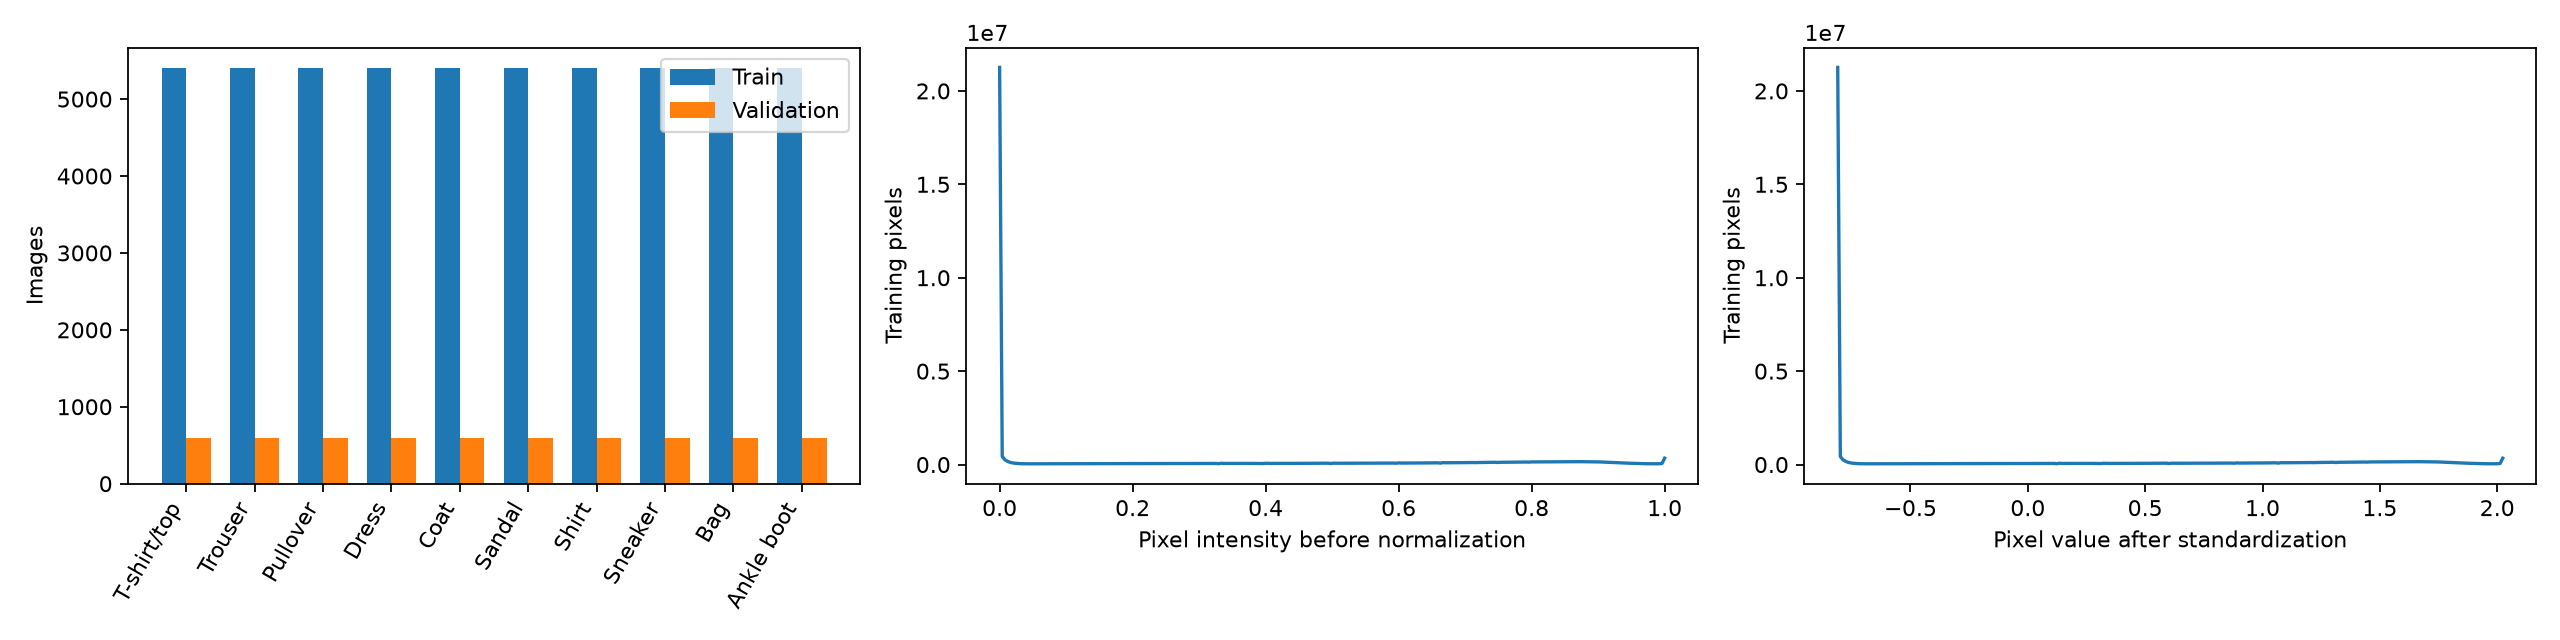
\includegraphics[width=0.7\textwidth,trim=0 0 756bp 0,clip]{notebook-evidence/figures/fashion_mnist_data_distribution.png}
\par\smallskip
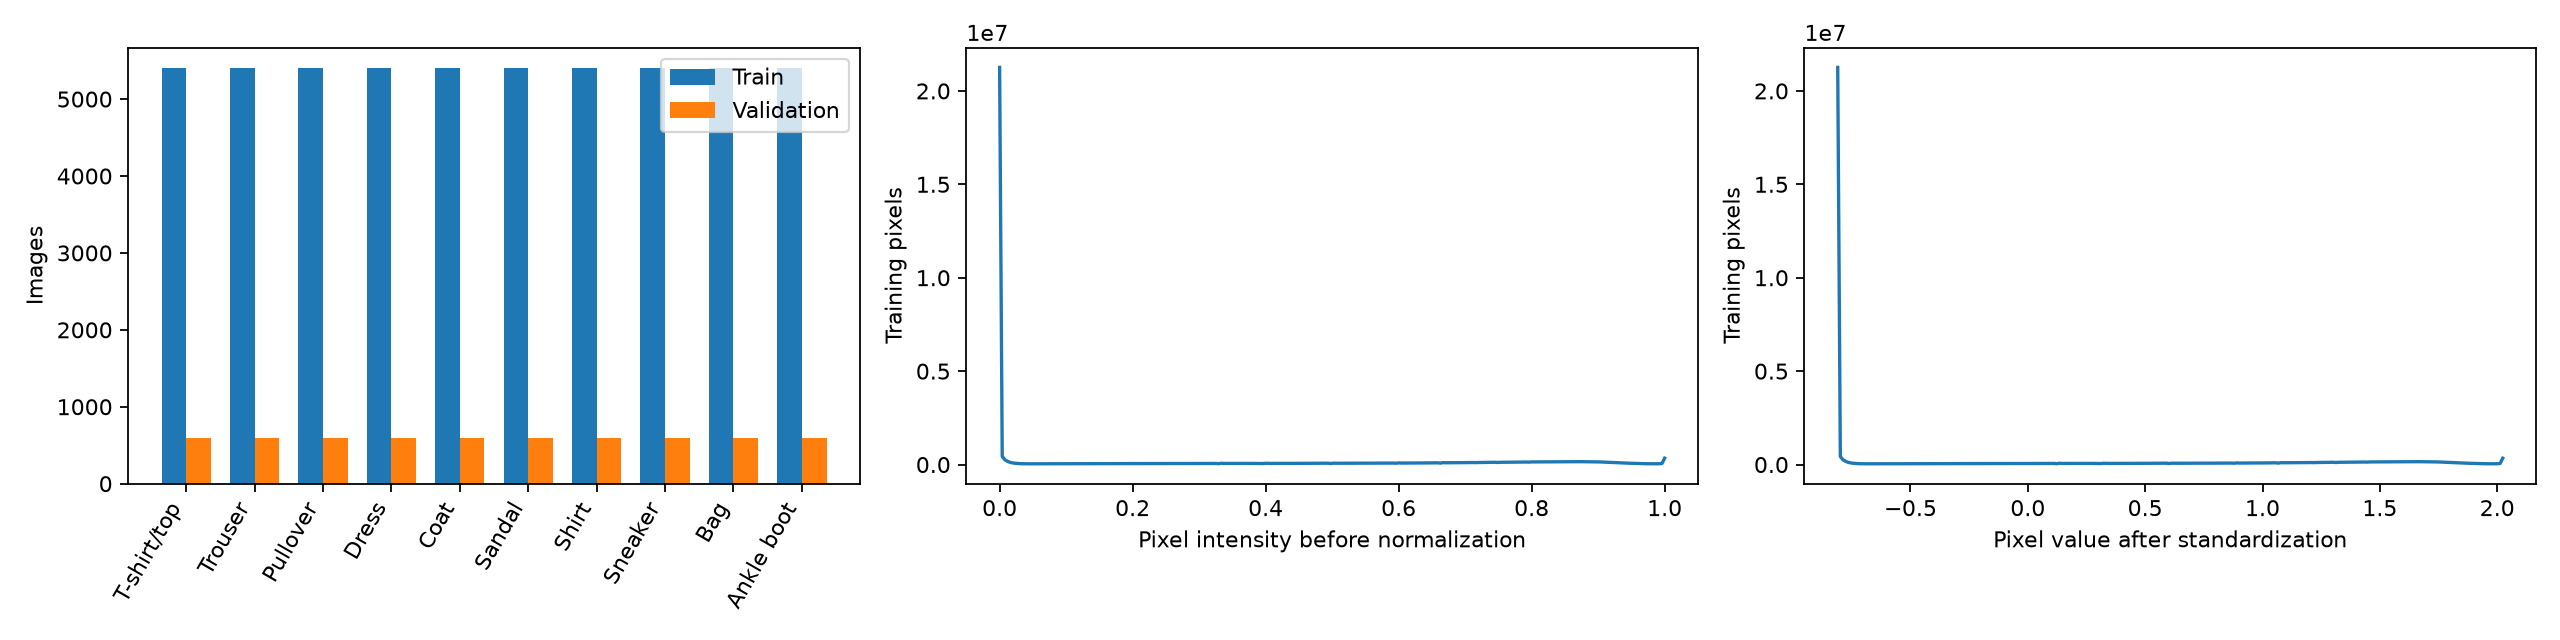
\includegraphics[width=\textwidth,trim=396bp 0 0 0,clip]{notebook-evidence/figures/fashion_mnist_data_distribution.png}
\caption{Trên: số ảnh train và validation theo lớp với phép chia seed 2026. Dưới: số pixel theo giá trị trước và sau chuẩn hóa, tính trên toàn bộ 54.000 ảnh train.}
\end{figure}

Ảnh minh họa gồm một ảnh train của mỗi lớp, chọn ngẫu nhiên với seed 2026. Ảnh chỉ có một kênh xám và ít chi tiết nhỏ. Các kiểu áo như T-shirt/top, Pullover, Coat và Shirt có thể có đường bao gần nhau; đây cũng là những lớp thường bị nhầm trong các kết quả phân loại bên dưới.

\resultfigure{fashion_mnist_training_examples}{Mỗi lớp một ảnh Fashion-MNIST từ tập train, chọn ngẫu nhiên với seed 2026.}{1.0}
\clearpage

\section{Huấn luyện và chỉ số đánh giá}
Mỗi mô hình xuất logits $z\in\R^{10}$, tức mười điểm số ứng với mười lớp. Softmax chuyển các điểm số thành xác suất $p_k$ của từng lớp. Huấn luyện dùng cross-entropy: loss lớn khi mô hình gán xác suất thấp cho nhãn đúng $y$.
\begin{equation}
\ell(z,y)=-z_y+\log\sum_{k=1}^{10}\exp(z_k),
\qquad \frac{\partial\ell}{\partial z_k}=p_k-\mathbf{1}[k=y].
\end{equation}
Cross-entropy được tính trực tiếp từ logits bằng log-softmax ổn định số. Softmax chỉ được dùng khi cần xác suất để trình bày dự đoán.

\begin{table}[htbp]\centering
\begin{tabularx}{\textwidth}{@{}lX@{}}\toprule
Tham số & Giá trị\\\midrule
Optimizer & AdamW, weight decay $10^{-4}$\\
Số epoch và batch size & 30 epoch; 256 ảnh/batch; không dừng sớm\\
Learning rate & E1/E3: $10^{-3}$; E2: $3\times10^{-4}$\\
Lịch learning rate & Giảm theo cosine đến 1\% giá trị ban đầu\\
Gradient clipping & Giới hạn chuẩn gradient toàn mô hình ở 1\\
Kiểu tính toán & FP32; không dùng AMP, TF32 hoặc compile\\
Seed huấn luyện & 42, 43 và 44\\
Chọn checkpoint & Accuracy validation cao nhất; nếu bằng nhau, chọn CE thấp hơn\\\bottomrule
\end{tabularx}
\caption{Thiết lập huấn luyện dùng chung cho E1–E3.}
\end{table}

Mọi mô hình đều train đủ 30 epoch với cùng batch size. AdamW cập nhật trọng số, còn weight decay hạn chế trọng số tăng quá lớn. Learning rate giảm theo cosine để các bước cập nhật nhỏ dần về cuối. Gradient clipping giới hạn độ lớn của gradient trước khi cập nhật. Learning rate được giữ giống nhau trong từng bài; báo cáo so sánh các mô hình theo thiết lập chung này, không tìm learning rate tốt nhất riêng cho từng mô hình.

Sau mỗi epoch, mô hình được đánh giá trên validation. Bộ trọng số có accuracy validation cao nhất được lưu làm checkpoint; nếu accuracy bằng nhau thì chọn CE thấp hơn. Train vẫn tiếp tục đủ 30 epoch, nên checkpoint được chọn có thể nằm trước epoch cuối. Chỉ sau khi chốt các cấu hình và hoàn tất train, checkpoint đã chọn mới được đánh giá trên test.

Accuracy là tỷ lệ ảnh được phân loại đúng. Macro-F1 tính F1 riêng cho từng lớp rồi lấy trung bình, giúp các lớp có vai trò ngang nhau trong chỉ số chung. Confusion matrix cho biết ảnh của từng lớp bị nhầm sang lớp nào; recall của một lớp là tỷ lệ ảnh lớp đó được nhận đúng. Các ảnh sai có confidence cao được xem thêm để nhận diện lỗi mà mô hình vẫn dự đoán tự tin.

Bảng kết quả ghi trung bình và độ lệch chuẩn mẫu qua ba seed. Đường cong học, confusion matrix và ảnh dự đoán sai dùng seed 42.

Chi phí được so sánh bằng số tham số và thời gian train mỗi epoch. Phép đo bao gồm tải batch và cập nhật trọng số; GPU được đồng bộ trước và sau khi đo để tính đúng thời gian thực thi. Với mỗi lượt, lấy trung vị từ epoch thứ hai trở đi để giảm ảnh hưởng của lần khởi tạo đầu tiên, rồi lấy trung bình qua ba seed. Các kết quả cho biết hiệu quả trong 30 epoch đã chọn.

\chapter{E1: Softmax, MLP và CNN}
\section{Ba bộ phân loại}
Softmax và MLP đều trải phẳng ảnh thành vector $x\in\R^{784}$. Bộ phân loại softmax tính logits bằng một phép biến đổi tuyến tính $z=Wx+b$. Với hai lớp $i,j$, ranh giới $z_i=z_j$ là một siêu phẳng. Vì không có tầng ẩn, mô hình chỉ học trọng số trực tiếp từ pixel đến lớp.

MLP dùng cùng vector ảnh nhưng thêm hai tầng ẩn với ReLU để học các quan hệ phi tuyến giữa pixel:
\begin{equation}
h_1=\operatorname{ReLU}(W_1x+b_1),\qquad
h_2=\operatorname{ReLU}(W_2h_1+b_2),\qquad z=W_3h_2+b_3.
\end{equation}
Dropout tạm đặt một phần giá trị tầng ẩn về 0 khi train, giúp mô hình bớt phụ thuộc vào một nhóm đặc trưng cố định. Phép flatten vẫn giữ mọi pixel, nhưng fully connected không khai thác riêng việc hai pixel nằm cạnh nhau trên ảnh.

CNN xử lý các vùng nhỏ trên ảnh. Mỗi kernel $3\times3$ dùng cùng một bộ trọng số ở nhiều vị trí, nhờ đó có thể nhận ra cùng một dạng đặc trưng ở các vùng khác nhau. Padding 1 giữ kích thước ảnh qua convolution. Max pooling lấy giá trị lớn nhất trong mỗi vùng $2\times2$ để giảm kích thước. Hình~\ref{fig:e1-architecture} cho thấy dữ liệu đi qua ba mô hình; bảng dưới liệt kê các lớp.

\ExerciseOneArchitecture

\begin{table}[htbp]\centering
\begin{tabularx}{\textwidth}{@{}lX@{}}\toprule
Mô hình & Các lớp theo thứ tự\\\midrule
Softmax & Flatten $784\to10$\\
MLP & Flatten; $784\to256$; ReLU; dropout 0,2; $256\to128$; ReLU; dropout 0,2; $128\to10$\\
CNN & Conv $1\to32$, kernel $3$, padding $1$; BN; ReLU; pool $2$; Conv $32\to64$ tương tự; pool $2$; flatten; $3136\to128$; ReLU; dropout 0,2; $128\to10$\\\bottomrule
\end{tabularx}
\caption{Kiến trúc E1. Conv không dùng bias vì sau đó có batch normalization.}
\end{table}

Hai phép pooling đưa ảnh $28\to14\to7$, vì vậy head CNN nhận $64\times7\times7=3136$ giá trị. Với một lớp Linear $d_{in}\to d_{out}$ có bias, số tham số là $d_{in}d_{out}+d_{out}$. Ví dụ softmax có $784\times10+10=7.850$ tham số. Số tham số của các mô hình gồm cả hệ số affine của batch normalization; các thống kê trung bình và phương sai tích lũy không phải tham số được học.

\section{Kết quả và phân tích lỗi}
\begin{table}[htbp]\centering\small
\begin{tabularx}{\textwidth}{@{}Xrrrr@{}}
\toprule
Mô hình & Tham số & Val (\%) & Test (\%) & Giây/epoch \\
\midrule
Softmax & 7,850 & 85.98 & 84.51 $\pm$ 0.15 & 0.29 \\
MLP & 235,146 & 91.02 & 89.88 $\pm$ 0.14 & 0.38 \\
CNN & 421,738 & 93.02 & 92.62 $\pm$ 0.06 & 0.48 \\
\bottomrule
\end{tabularx}

\caption{Kết quả E1 qua ba seed 42, 43 và 44.}
\end{table}
\tablenote

\subsection{Accuracy, macro-F1 và loss của ba mô hình}
MLP đạt accuracy test 89,85\%, tăng 5,25 điểm phần trăm so với 84,60\% của softmax. Các tầng ẩn giúp MLP học những quan hệ giữa pixel mà một phép biến đổi tuyến tính không biểu diễn được.

CNN đạt 92,66\%, cao hơn MLP 2,80 điểm phần trăm. Kết quả này phù hợp với lợi ích của việc học đặc trưng từ các vùng lân cận trên ảnh. Tuy nhiên, CNN cũng có nhiều tham số hơn MLP, nên thí nghiệm không đo riêng tác động của convolution.

Thứ tự CNN, MLP, softmax giữ nguyên khi xét macro-F1, với giá trị trung bình tương ứng 0,9262, 0,8983 và 0,8443. Độ lệch chuẩn accuracy qua ba seed của softmax, MLP và CNN lần lượt là 0,05, 0,08 và 0,11 điểm phần trăm. Biến thiên giữa các lượt nhỏ hơn khoảng cách accuracy giữa các mô hình.

Ở epoch cuối, CNN đạt accuracy train trung bình 99,50\%, nhưng accuracy validation chỉ đạt 92,89\%. CE tương ứng là 0,0190 và 0,2852. Mô hình gần như nhận đúng toàn bộ ảnh train trong khi vẫn còn lỗi trên ảnh chưa dùng để cập nhật trọng số. Đây là dấu hiệu overfitting.

MLP cũng có khoảng cách CE train--validation, ở mức 0,1398/0,2879; softmax có khoảng cách nhỏ hơn, ở mức 0,3668/0,4059. CE train cao của softmax đi cùng accuracy thấp hơn, cho thấy mô hình tuyến tính còn hạn chế trong việc khớp dữ liệu. Các đường cong bên dưới giúp theo dõi sự khác nhau này qua từng epoch ở seed 42.

Ba checkpoint CNN được chọn ở epoch 19, 23 và 26, đều trước epoch cuối. Việc lưu checkpoint theo validation giúp chọn trọng số hoạt động tốt trên dữ liệu ngoài tập train, thay vì chỉ chọn trọng số khớp train nhất.

\subsection{Các lỗi thường gặp}
Confusion matrix CNN ở seed 42 cho thấy Shirt là lớp khó nhất, với recall 73,2\%. Có 98 ảnh Shirt bị nhận thành T-shirt/top và 68 ảnh nhầm theo chiều ngược lại. Shirt còn bị nhầm thành Pullover ở 74 ảnh và Coat ở 65 ảnh. Các lớp này đều là áo và có thể có hình dáng gần nhau trong ảnh nhỏ.

Ngược lại, recall của Trouser, Sandal, Sneaker và Bag đều trên 98\%. Lỗi vì vậy tập trung vào một số kiểu trang phục, không phân bố đều giữa các lớp. Hình ảnh sai bên dưới bổ sung ví dụ cụ thể: mô hình có thể đưa ra confidence cao dù chọn sai lớp. Confidence cao ở một dự đoán không bảo đảm dự đoán đó đúng.

\subsection{Chi phí huấn luyện}
Trên cùng RTX 5090 với DataLoader không dùng worker, CNN cần khoảng 0,96 giây/epoch, MLP cần 0,83 và softmax cần 0,78. CNN có khoảng 1,79 lần số tham số MLP, nhưng thời gian mỗi epoch chỉ cao hơn khoảng 15,4\%. Trong thiết lập này, mức tăng thời gian đó đi cùng mức tăng 2,80 điểm phần trăm accuracy.

Tổng thời gian train của chín lượt là khoảng 233 giây, không gồm validation, test và vẽ hình. Phép đo cho thấy số tham số và thời gian không tăng cùng tỷ lệ: thời gian còn phụ thuộc loại phép tính và cách GPU thực thi chúng.

\resultfigure{e1_comparison_ce}{CE train và validation của ba mô hình E1 ở seed 42.}{0.88}
\resultfigure{e1_comparison_accuracy}{Accuracy train và validation của ba mô hình E1 ở seed 42.}{0.88}
\resultfigure{e1_cnn_confusion}{Confusion matrix test của CNN ở seed 42; mỗi hàng có 1.000 ảnh, các ô ghi số ảnh.}{0.9}
\resultfigure{e1_cnn_mistakes}{Tám dự đoán sai có confidence cao nhất của CNN trên tập test ở seed 42.}{0.95}

\chapter{E2: MSA và cách lấy token}
\section{Hiện thực attention}
Self-attention cho phép mỗi token kết hợp thông tin từ các token khác trong cùng ảnh. Đầu vào là tensor $X\in\R^{B\times N\times d}$, trong đó $B$ là batch size, $N$ là số token và $d$ là số chiều của mỗi token. Mỗi head biến đổi đầu vào thành query $Q$, key $K$ và value $V$. Bỏ chỉ số batch để gọn, attention của một head được tính như sau \cite{attention}:
\begin{equation}
Q=XW_Q,\quad K=XW_K,\quad V=XW_V,\qquad
A=\operatorname{softmax}_{\text{hàng}}\left(\frac{QK^\top}{\sqrt{d_h}}\right),\quad O=AV.
\end{equation}
Mỗi phần tử của $QK^\top$ là điểm số giữa một query và một key. Phép chia cho $\sqrt{d_h}$, với $d_h$ là số chiều mỗi head, giữ điểm số không tăng quá lớn khi số chiều tăng. Softmax biến các điểm số thành trọng số có tổng bằng 1 theo chiều key. Cuối cùng, $O=AV$ lấy tổng có trọng số của các value. Nhờ đó, đầu ra của một token có thể sử dụng thông tin ở mọi vị trí trên ảnh.

Trong bài này, $d=64$ và có bốn head nên $d_h=16$. Mỗi head dùng các phép chiếu riêng để tính attention. Kết quả các head được ghép lại rồi qua phép chiếu đầu ra để trở về số chiều ban đầu. Bias có trong mô hình nhưng được lược khỏi công thức để dễ đọc.

Bản MSA tự viết gồm các phép Linear, tách head, nhân ma trận, softmax, dropout và ghép head. Các phép tính attention được thực hiện trực tiếp bằng những thao tác này.

Bản đối chiếu dùng multi-head attention của PyTorch. Với mỗi seed, hai phiên bản bắt đầu từ cùng trọng số, từ tokenizer đến MSA và head phân loại. Cách ghép cặp này giúp so sánh hai cách hiện thực attention trên cùng điểm xuất phát. Khi train, dropout và các kernel khác nhau vẫn có thể dẫn đến quá trình cập nhật khác nhau.

Hình~\ref{fig:e2-manual-msa} trình bày thứ tự các phép tính trong MSA tự viết. Phép chiếu QKV được tính chung trước khi tách bốn head; mỗi head tính softmax riêng. Sau khi ghép head, output projection tạo đầu ra cuối cùng của khối MSA.

\ExerciseTwoAttention

\section{Ba cách tokenization}
Tokenization là bước chuyển ảnh thành các vector để đưa vào attention. Ba cách dưới đây khác nhau ở phần ảnh mà mỗi token chứa và ở việc có học đặc trưng cục bộ trước attention hay không.
\begin{table}[htbp]\centering
\begin{tabularx}{\textwidth}{@{}lrrX@{}}\toprule
Cách chia & $N$ & Đầu vào/token & Phép tạo embedding\\\midrule
Hàng & 28 & 28 & Linear $28\to64$\\
Patch $4\times4$ & 49 & 16 & Unfold không chồng lấp, Linear $16\to64$\\
CNN-stem & 49 & 64 & Hai Conv stride 2: $1\to32\to64$, BN/ReLU; flatten spatial\\\bottomrule
\end{tabularx}
\caption{Tokenization của E2 trên ảnh $1\times28\times28$.}
\end{table}

Với token hàng, mỗi vector chứa các pixel của một hàng ảnh. Với token patch, ảnh được chia thành các ô $4\times4$ không chồng lấp; các ô được đọc từ trái sang phải rồi xuống hàng tiếp theo. Hai cách này đưa pixel trực tiếp qua Linear để tạo embedding.

CNN-stem xử lý ảnh bằng convolution trước, tạo feature map $64\times7\times7$. Mỗi vị trí trên feature map trở thành một token chứa đặc trưng cục bộ đã học. Stem cũng được train từ đầu, vì vậy cách này cần thêm tham số và phép tính.

Hình~\ref{fig:e2-tokenizers} cho thấy ba cách chuyển cùng một ảnh thành chuỗi. Số chiều embedding đều là 64, trong khi số token phụ thuộc cách biểu diễn.

\ExerciseTwoTokenizers

Positional embedding được học và cộng vào từng token để đánh dấu vị trí trên ảnh. Nếu chỉ dùng attention rồi mean pooling, mô hình không phân biệt được hai chuỗi chỉ khác thứ tự các token. Positional embedding bổ sung thông tin còn thiếu này.

Sau bước tạo token, mỗi cấu hình dùng hai encoder block dạng pre-LN. Đầu ra đi qua LayerNorm, mean pooling và Linear $64\to10$ để phân loại. Mô hình không dùng CLS token. Mỗi block tính
\begin{align}
U &= X+\operatorname{Dropout}(\operatorname{MSA}(\operatorname{LN}(X))),\\
Y &= U+\operatorname{FFN}(\operatorname{LN}(U)),
\end{align}
trong đó FFN là $64\to128\to64$ với GELU và dropout 0,1. $\operatorname{LN}$ là LayerNorm, được đặt trước MSA và FFN. Hai phép cộng giữ đường truyền trực tiếp từ đầu vào bên cạnh kết quả biến đổi của mỗi nhánh; đây là residual connection. Attention không dùng causal mask vì mô hình được phép sử dụng toàn bộ ảnh để phân loại.

Hình~\ref{fig:e2-encoder} đặt encoder block trong mô hình phân loại hoàn chỉnh. Hai block có cùng cấu trúc nhưng không dùng chung trọng số. Mean pooling lấy trung bình theo chiều token để tạo một vector 64 chiều cho lớp phân loại cuối.

\ExerciseTwoEncoder

\section{So sánh attention và tokenization}
\begin{table}[htbp]\centering\small
\begin{tabularx}{\textwidth}{@{}Xrrrr@{}}
\toprule
Mô hình & Tham số & Val (\%) & Test (\%) & Giây/epoch \\
\midrule
Hàng / tự viết & 71.370 & 88,52 & 87,96 $\pm$ 0,16 & 1,31 \\
Hàng / PyTorch & 71.370 & 88,52 & 87,99 $\pm$ 0,16 & 1,31 \\
Patch / tự viết & 71.946 & 86,27 & 86,02 $\pm$ 0,13 & 1,45 \\
Patch / PyTorch & 71.946 & 86,38 & 86,02 $\pm$ 0,15 & 1,46 \\
CNN-stem / tự viết & 89.770 & 89,04 & 88,70 $\pm$ 0,61 & 1,37 \\
CNN-stem / PyTorch & 89.770 & 89,11 & 88,64 $\pm$ 0,33 & 1,37 \\
\bottomrule
\end{tabularx}

\caption{Sáu cấu hình E2. Manual và PyTorch của cùng tokenizer có cùng số tham số.}
\end{table}
\tablenote

\subsection{Hai cách hiện thực MSA}
Với mỗi tokenizer, bản tự viết được so sánh với bản PyTorch. Các phần còn lại của mô hình và cách train được giữ giống nhau. Mục đích là xem việc thay cách hiện thực MSA ảnh hưởng thế nào đến accuracy và thời gian train.

Hai bản có accuracy trung bình gần nhau ở cả ba tokenizer. Bảng dưới lấy kết quả PyTorch trừ kết quả tự viết ở từng seed, rồi tính trung bình và SD. Chênh lệch accuracy trung bình lớn nhất chỉ là 0,06 điểm phần trăm; dấu của chênh lệch còn thay đổi giữa các seed. Kết quả không cho thấy một cách hiện thực luôn đạt accuracy cao hơn.

\begin{table}[htbp]\centering\small
\begin{tabularx}{\textwidth}{@{}Xrrr@{}}
\toprule
Tokenizer & $\Delta$ accuracy (đpt) & $\Delta$ giây/epoch & GPU peak (MiB) \\
\midrule
Hàng & +0,03 $\pm$ 0,12 & -0,004 $\pm$ 0,017 & 87,96 / 82,17 \\
Patch & +0,00 $\pm$ 0,05 & +0,013 $\pm$ 0,016 & 158,26 / 121,30 \\
CNN-stem & -0,06 $\pm$ 0,30 & -0,001 $\pm$ 0,054 & 176,08 / 139,12 \\
\bottomrule
\end{tabularx}

\caption{So sánh hai cách hiện thực MSA qua ba seed. $\Delta$ là PyTorch trừ bản tự viết, ghi trung bình $\pm$ SD; đpt là điểm phần trăm. Cột GPU peak ghi trung bình bộ nhớ tensor lớn nhất khi train, theo thứ tự tự viết / PyTorch.}
\end{table}

Thời gian train mỗi epoch của hai bản gần nhau, không có xu hướng bản PyTorch luôn nhanh hơn. Phép đo tính cho toàn bộ mô hình, gồm cả tokenizer và FFN. Trong khi đó, PyTorch có GPU peak thấp hơn ở cả ba tokenizer. GPU peak ở đây chỉ tính bộ nhớ tensor đã cấp phát trong quá trình train, không phải toàn bộ bộ nhớ GPU mà hệ thống sử dụng.

\subsection{Ba cách tạo token}
CNN-stem đạt accuracy test 88,70\% với MSA tự viết và 88,64\% với MSA PyTorch, cao nhất trong mỗi nhóm. Ở bản tự viết, CNN-stem cao hơn token hàng 0,74 điểm phần trăm và cao hơn patch 2,68 điểm phần trăm. Convolution giúp các token chứa đặc trưng của vùng ảnh trước khi attention kết hợp chúng. Đây là khác biệt chính so với việc đưa pixel qua Linear ở hai tokenizer còn lại.

Macro-F1 của bản tự viết cũng xếp CNN-stem cao nhất, ở mức 0,8868, tiếp theo là token hàng 0,8793 và patch 0,8602. Tuy nhiên, accuracy của CNN-stem biến thiên giữa các seed nhiều hơn hai cách tạo token còn lại, như SD trong bảng cho thấy.

Số token cũng ảnh hưởng chi phí. Attention phải tính điểm cho mọi cặp token, với chi phí tỉ lệ $N^2d$. Patch có số cặp token gấp $49^2/28^2\approx3,06$ lần token hàng. Trong bản tự viết, token hàng cần khoảng 1,31 giây/epoch, patch cần 1,45 và CNN-stem cần 1,37. Chia ảnh thành các vùng nhỏ hơn không tự động làm mô hình nhanh hơn. Thời gian thực tế còn gồm các phép chiếu, FFN và CNN-stem.

Trong các cấu hình đã thử, cả ba cách tạo token vẫn có accuracy thấp hơn MLP và CNN của E1. Kết quả này giới hạn ở các mô hình nhỏ, train từ đầu trong 30 epoch; không đại diện cho mọi mô hình attention dùng trong phân loại ảnh.

\subsection{CE train/validation và lỗi theo lớp}
Ở epoch cuối, MSA tự viết với CNN-stem có CE train/validation trung bình là 0,2565/0,3162. Bản dùng patch có CE cao hơn ở cả hai tập, 0,3541/0,3721. Khoảng cách train--validation của patch nhỏ nhưng accuracy vẫn thấp hơn. Điều này gợi ý bản dùng patch còn hạn chế trong việc khớp dữ liệu với thiết lập đã chọn, thay vì chỉ gặp vấn đề overfitting.

Hình train/validation dưới đây tách riêng hai bản CNN-stem ở seed 42. Hai đường CE train gần trùng nhau; CE validation cũng nằm gần nhau trong phần lớn quá trình học. Từ epoch 20 đến 30, CE train và validation còn giảm ở cả hai bản. Vì vậy, hình này chưa cho thấy validation xấu dần rõ rệt về cuối, dù khoảng cách với train vẫn tồn tại. CE train/validation ở epoch cuối là 0,2555/0,3187 với bản tự viết và 0,2554/0,3133 với PyTorch.

\resultfigure{e2_cnn_train_validation_ce}{CE train và validation của MSA tự viết và MSA PyTorch dùng CNN-stem ở seed 42.}{0.95}

Trong confusion matrix của MSA tự viết với CNN-stem ở seed 42, Shirt có recall 68,1\%. Có 133 ảnh T-shirt/top bị nhận thành Shirt, 103 ảnh nhầm theo chiều ngược lại và 112 ảnh Shirt bị nhận thành Coat. Các lớp Trouser và Bag đều có recall 96,7\%. Tương tự E1, lỗi tập trung vào những kiểu áo gần nhau về hình dáng. Hình dự đoán sai cho thấy một số ảnh vẫn được gán confidence cao dù sai lớp.

\resultfigure{e2_comparison_ce}{Validation CE của sáu cấu hình E2 ở seed 42.}{0.9}
\resultfigure{e2_comparison_accuracy}{Validation accuracy của sáu cấu hình E2 ở seed 42.}{0.9}
\resultfigure{e2_cnn_manual_confusion}{Confusion matrix test của MSA tự viết dùng CNN-stem ở seed 42; các ô ghi số ảnh.}{0.9}
\resultfigure{e2_cnn_manual_mistakes}{Tám dự đoán sai có confidence cao nhất của MSA tự viết dùng CNN-stem trên tập test ở seed 42.}{0.95}

\chapter{E3: LSTM/GRU trên chuỗi ảnh}
\section{Biểu diễn ảnh và kiến trúc}
LSTM và GRU nhận từng phần của ảnh theo thứ tự. Với cách đọc theo hàng, mô hình nhận hàng trên cùng trước, rồi lần lượt đến hàng dưới cùng: chuỗi có $T=28$ bước, mỗi bước chứa $D=28$ pixel. Với patch $4\times4$, các ô được đọc từ trái sang phải rồi xuống hàng tiếp theo, tạo chuỗi $T=49,D=16$. Pixel được đưa trực tiếp vào RNN, không qua embedding học được.

Cả LSTM và GRU đều có một tầng, chỉ đọc theo một chiều và dùng hidden size $H=128$. Hidden state là vector được cập nhật sau mỗi token để mang thông tin từ các token đã đọc. Trạng thái ban đầu bằng zero. Sau token cuối, hidden state đi qua dropout 0,1 rồi Linear $128\to10$ để phân loại ảnh.

Token hàng chứa trọn một hàng ảnh, còn token patch chỉ chứa một vùng nhỏ. Do đó, khi đổi cách đọc, cả nội dung mỗi token lẫn số bước xử lý đều thay đổi.

Hình~\ref{fig:e3-architecture} cho thấy mô hình xử lý lần lượt các token. Mọi bước dùng chung trọng số và hidden size 128. LSTM truyền cả hidden state và cell state sang bước tiếp theo; GRU chỉ dùng hidden state. Các gate quyết định giữ bao nhiêu thông tin cũ và thêm bao nhiêu thông tin mới.

\ExerciseThreeArchitecture

\section{Các phương trình được sử dụng}
Tại bước $t$, LSTM nhận token $x_t$ và trạng thái từ bước trước. Đặt $a_t=W_xx_t+W_hh_{t-1}+b$ rồi tách thành bốn phần \cite{pytorch-lstm}:
\begin{align}
i_t&=\sigma(a_t^i),& f_t&=\sigma(a_t^f),& g_t&=\tanh(a_t^g),& o_t&=\sigma(a_t^o),\\
c_t&=f_t\odot c_{t-1}+i_t\odot g_t,&&
h_t=o_t\odot\tanh(c_t).
\end{align}
Trong các phương trình, $\sigma$ là sigmoid, $\tanh$ là hyperbolic tangent và $\odot$ là phép nhân theo từng phần tử. Forget gate $f_t$ quyết định phần cell state cũ $c_{t-1}$ được giữ lại. Input gate $i_t$ quyết định phần thông tin mới $g_t$ được thêm vào. Output gate $o_t$ điều tiết thông tin từ cell state $c_t$ sang hidden state $h_t$.

Cell state tạo một đường truyền trực tiếp từ bước trước đến bước sau. Trên đường này, đạo hàm theo cell state trước là $f_t$; qua nhiều bước, đạo hàm chứa tích các forget gate. Các giá trị gần 1 giúp gradient truyền qua đường này. Tuy vậy, toàn bộ gradient còn đi qua các gate và hidden state, nên cơ chế đó không bảo đảm gradient luôn được giữ nguyên.

GRU dùng reset gate $r_t$, update gate $z_t$ và trạng thái ứng viên $n_t$. Các phương trình trong mô hình tuân theo cách định nghĩa của PyTorch \cite{pytorch-gru}:
\begin{align}
r_t &=\sigma(W_{ir}x_t+b_{ir}+W_{hr}h_{t-1}+b_{hr}),\\
z_t &=\sigma(W_{iz}x_t+b_{iz}+W_{hz}h_{t-1}+b_{hz}),\\
n_t &=\tanh\!\left(W_{in}x_t+b_{in}+r_t\odot(W_{hn}h_{t-1}+b_{hn})\right),\\
h_t &=(1-z_t)\odot n_t+z_t\odot h_{t-1}.
\end{align}
Update gate $z_t$ quyết định tỷ lệ hidden state cũ được giữ lại khi tạo $h_t$. Reset gate $r_t$ điều tiết thông tin từ hidden state cũ để tính trạng thái ứng viên $n_t$. Trong công thức PyTorch, reset gate được nhân sau phép chiếu hidden, khác với cách viết $W_{hn}(r_t\odot h_{t-1})$.

GRU chỉ dùng hidden state, trong khi LSTM có thêm cell state. GRU tính ba nhóm phép chiếu, ít hơn bốn nhóm của LSTM. Vì vậy, khi giữ cùng kích thước đầu vào và hidden size, GRU cần ít tham số hơn.

PyTorch lưu hai vector bias cho mỗi tầng. Tính cả các bias này, phần recurrent có $4H(D+H+2)$ tham số ở LSTM và $3H(D+H+2)$ ở GRU. Head phân loại thêm $10H+10$ tham số. Các công thức này giải thích vì sao hai mô hình cùng $H$ vẫn có số tham số khác nhau trong bảng kết quả.

\section{Kết quả phân loại}
\begin{table}[htbp]\centering\small
\begin{tabularx}{\textwidth}{@{}Xrrrr@{}}
\toprule
Mô hình & Tham số & Val (\%) & Test (\%) & Giây/epoch \\
\midrule
MLP & 235.146 & 90,53 & 90,02 $\pm$ 0,07 & 0,85 \\
CNN & 421.738 & 92,98 & 92,48 $\pm$ 0,27 & 0,96 \\
LSTM / hàng & 82.186 & 90,01 & 89,37 $\pm$ 0,16 & 0,91 \\
GRU / hàng & 61.962 & 90,37 & 90,17 $\pm$ 0,12 & 0,88 \\
LSTM / patch & 76.042 & 88,26 & 87,76 $\pm$ 0,07 & 1,17 \\
GRU / patch & 57.354 & 88,73 & 88,19 $\pm$ 0,32 & 1,13 \\
\bottomrule
\end{tabularx}

\caption{Kết quả E3 qua ba seed 42, 43 và 44; MLP và CNN được huấn luyện riêng trong E3.}
\end{table}
\tablenote

\subsection{Ảnh hưởng của cách đọc ảnh}
CNN xử lý trực tiếp các vùng lân cận hai chiều. LSTM và GRU nhận lần lượt từng token, nên vị trí trong chuỗi quyết định phần nào của ảnh được xử lý trước. Với patch, token cuối một hàng nối sang token đầu hàng kế tiếp dù hai vùng này có thể cách xa nhau trên ảnh. Hai cách đọc vì vậy tạo ra quan hệ khác nhau giữa các token liên tiếp.

Cả LSTM và GRU đều đạt accuracy test cao hơn khi đọc theo hàng. Để so sánh, ở mỗi seed lấy accuracy của bản theo hàng trừ bản theo patch, rồi tính trung bình và SD của các chênh lệch. Kết quả là $1{,}60\pm0{,}18$ điểm phần trăm ở LSTM và $1{,}99\pm0{,}35$ ở GRU. Trong thiết lập này, đọc trọn một hàng ảnh hiệu quả hơn đọc các patch nhỏ theo chuỗi dài hơn.

Khi cùng đọc theo hàng, GRU cao hơn LSTM $0{,}81\pm0{,}21$ điểm phần trăm. Macro-F1 cũng cao hơn, ở mức 0,9015 so với 0,8933. Như vậy, GRU dùng ít tham số hơn nhưng vẫn phân loại tốt hơn LSTM trong so sánh này.

\subsection{So sánh với MLP và CNN}
GRU theo hàng đạt accuracy 90,17\%, gần với MLP (90,02\%) và thấp hơn CNN (92,48\%). MLP và CNN trong bảng được train riêng trong E3; đây không phải số liệu dùng lại từ E1.

Theo cách tính chênh lệch ở từng seed, GRU hơn MLP $0{,}16\pm0{,}06$ điểm phần trăm. Chênh lệch accuracy nhỏ, trong khi GRU chỉ có 61.962 tham số, bằng khoảng 26\% số tham số MLP.

CNN cao hơn GRU $2{,}31\pm0{,}25$ điểm phần trăm nhưng cần 421.738 tham số; GRU chỉ dùng khoảng 15\% số tham số đó. GRU vì vậy là lựa chọn ít tham số hơn khi chấp nhận accuracy thấp hơn CNN trong bài này.

GRU theo hàng cần khoảng 0,88 giây/epoch, gần MLP (0,85) và thấp hơn CNN (0,96). GRU dùng ít tham số hơn MLP nhưng không nhanh hơn trong phép đo này. Hai mô hình thực hiện các phép tính khác nhau: GRU xử lý lần lượt các token, còn MLP xử lý toàn bộ vector ảnh qua các lớp fully connected.

Bản GRU theo patch cần 1,13 giây/epoch. LSTM cũng có cùng xu hướng: 0,91 giây/epoch khi đọc theo hàng và 1,17 khi đọc theo patch. Chuỗi patch có 49 bước thay vì 28, nên mô hình phải cập nhật trạng thái nhiều lần hơn. Tuy nhiên, kích thước đầu vào và số tham số cũng thay đổi, nên không thể quy toàn bộ chênh lệch cho độ dài chuỗi.

\subsection{CE train/validation và lỗi theo lớp}
Ở epoch cuối, CE train/validation trung bình của GRU theo hàng là 0,1805/0,2783. LSTM theo hàng có CE train thấp hơn, 0,1648, nhưng CE validation cao hơn, 0,2924. LSTM khớp tập train tốt hơn mà không cải thiện kết quả trên validation. Có thêm tham số chưa đem lại lợi thế trong lần so sánh này.

Với token patch, CE train/validation là 0,2447/0,3360 ở LSTM và 0,2463/0,3208 ở GRU. Cả bốn cấu hình đều có CE validation cao hơn CE train. Các bảng test vẫn sử dụng checkpoint được chọn trên validation, không mặc định lấy epoch cuối.

Ở seed 42, hình train/validation cho thấy CE train của cả LSTM và GRU tiếp tục giảm trong đoạn cuối, còn CE validation gần như đi ngang. LSTM có CE validation thấp nhất ở epoch 20, bằng 0,2816, rồi tăng nhẹ lên 0,2860 ở epoch cuối. Việc khớp train tốt hơn không còn cải thiện validation ở đoạn này, cho thấy dấu hiệu overfitting. GRU có CE train cao hơn LSTM ở cuối nhưng CE validation thấp hơn, cùng xu hướng với kết quả trung bình qua ba seed.

\resultfigure{e3_rows_train_validation_ce}{CE train và validation của LSTM và GRU đọc ảnh theo hàng ở seed 42.}{0.95}

Confusion matrix của GRU theo hàng ở seed 42 cho thấy Shirt có recall 71,0\%. Có 134 ảnh Shirt bị nhận thành T-shirt/top và 82 ảnh nhầm theo chiều ngược lại. Ngoài ra, 83 ảnh Coat bị nhận thành Pullover. Các kiểu áo này cũng gây nhầm lẫn cho CNN trong E1. Cách đọc theo hàng cải thiện accuracy so với patch nhưng vẫn gặp khó khăn khi phân biệt các kiểu áo gần nhau trên ảnh $28\times28$.

\resultfigure{e3_comparison_ce}{Validation CE của LSTM, GRU, MLP và CNN trong E3 ở seed 42.}{0.9}
\resultfigure{e3_comparison_accuracy}{Validation accuracy của LSTM, GRU, MLP và CNN trong E3 ở seed 42.}{0.9}
\resultfigure{e3_gru_rows_confusion}{Confusion matrix test của GRU đọc theo hàng ở seed 42; các ô ghi số ảnh.}{0.9}

\clearpage
\section{Ảnh hưởng của thứ tự token đến LSTM và GRU}
\subsection{Thay đổi thứ tự đầu vào sau khi huấn luyện}
Khi train, LSTM và GRU luôn nhận token theo một thứ tự cố định: các hàng ảnh đi từ trên xuống dưới; các patch đi từ trái sang phải rồi xuống hàng tiếp theo. Phép thử dưới đây kiểm tra dự đoán thay đổi ra sao khi giữ nguyên ảnh nhưng đổi thứ tự đưa token vào mô hình.

Các checkpoint đã chọn bằng validation được đánh giá trên cùng 256 ảnh validation. Trọng số được giữ nguyên, chỉ thay cách sắp xếp token:
\begin{itemize}
\item \textbf{Thứ tự gốc:} đưa token vào đúng thứ tự đã dùng khi train.
\item \textbf{Đảo ngược:} đưa token cuối vào trước, rồi lần lượt trở về token đầu. Với cách đọc theo hàng, mô hình nhận hàng dưới cùng trước thay vì hàng trên cùng.
\item \textbf{Hoán vị cố định:} sắp xếp lại các token theo một thứ tự ngẫu nhiên tạo với seed 2026. Cùng một thứ tự được áp dụng cho mọi ảnh có cùng cách tokenization.
\end{itemize}

\begin{table}[htbp]\centering\small
\begin{tabularx}{\textwidth}{@{}Xrrr@{}}
\toprule
Mô hình & Gốc (\%) & Đảo ngược (\%) & Hoán vị (\%) \\
\midrule
LSTM / hàng & 90,76 $\pm$ 0,81 & 25,65 $\pm$ 4,07 & 41,93 $\pm$ 4,10 \\
GRU / hàng & 90,62 $\pm$ 1,17 & 20,18 $\pm$ 1,63 & 41,67 $\pm$ 1,93 \\
LSTM / patch & 87,37 $\pm$ 0,23 & 18,10 $\pm$ 3,32 & 13,15 $\pm$ 1,63 \\
GRU / patch & 87,89 $\pm$ 1,41 & 17,58 $\pm$ 3,12 & 13,54 $\pm$ 4,44 \\
\bottomrule
\end{tabularx}

\caption{Accuracy trên cùng 256 ảnh validation với ba thứ tự token; trung bình $\pm$ SD qua seed 42, 43 và 44.}
\end{table}

Ví dụ, LSTM đọc theo hàng đạt accuracy 90,76\% ở thứ tự gốc, nhưng chỉ còn 25,65\% khi đọc từ hàng cuối lên hàng đầu và 41,93\% khi hoán vị các hàng. Cả bốn cấu hình đều giảm accuracy khi đổi thứ tự. Kết quả cho thấy mô hình đã thích nghi với cách sắp xếp token trong tập train; thứ tự đầu vào là một phần quan trọng của biểu diễn ảnh. Các mô hình không được train lại sau khi đổi thứ tự, nên đây là phép kiểm tra trên checkpoint hiện có.

\subsection{Gradient của loss theo từng vị trí token}
Phép đo thứ hai xem loss thay đổi như thế nào trước một biến đổi nhỏ ở từng token đầu vào. Với $M=256$ ảnh, $\ell_i$ là cross-entropy của ảnh $i$ và $x_{i,t}$ là token ở vị trí $t$, chuẩn gradient trung bình được tính bằng
\begin{equation}
g_t=\frac{1}{M}\sum_{i=1}^{M}\left\|\frac{\partial\ell_i}{\partial x_{i,t}}\right\|_2.
\end{equation}
$g_t$ lớn cho biết loss có thể thay đổi mạnh hơn khi token tại vị trí đó bị biến đổi nhỏ. Gradient được tính đối với token đầu vào của từng ảnh, rồi lấy trung bình trên 256 ảnh; khi hiện thực, cross-entropy được cộng trên batch để không làm gradient bị chia thêm cho batch size.

Ở LSTM đọc theo hàng với seed 42, $g_t$ bằng 0,2152 ở hàng đầu, giảm đến 0,0398 ở hàng 17 rồi tăng lên 0,0826 ở hàng cuối. Đường cong không giảm đều theo khoảng cách đến cuối chuỗi. Các giá trị này mô tả phản ứng của loss trên nhóm ảnh đang xét; chúng chưa đủ để kết luận mô hình học được phụ thuộc dài hạn hay bị vanishing gradient.

\resultfigure{e3_sequence_diagnostics}{Trên: accuracy khi đổi thứ tự token, trung bình $\pm$ SD qua seed 42, 43 và 44. Dưới: chuẩn gradient của cross-entropy theo vị trí token ở seed 42. Cả hai phép đo dùng cùng 256 ảnh validation.}{0.92}

\chapter{Phạm vi thực nghiệm và giới hạn}
\label{chap:ta-lap}
\section{Cấu hình và các lượt chạy}
Ba notebook đã hoàn tất 45 lượt train và 45 lượt đánh giá test, gồm 15 cấu hình với ba seed mỗi cấu hình. Hai baseline MLP và CNN được train riêng trong E3, với cùng cách chia dữ liệu và siêu tham số như E1.

Cả ba bài chạy trên RTX 5090 với PyTorch 2.10.0, FP32 và DataLoader không dùng worker. Mỗi lượt có đủ 30 epoch và 10.000 dự đoán test. Các bảng và hình trong báo cáo sử dụng kết quả của những lượt này.

\begin{table}[htbp]\centering
\begin{tabularx}{\textwidth}{@{}lXrr@{}}\toprule
Bài & Cấu hình & Số cấu hình & Số lượt\\\midrule
E1 & Softmax, MLP, CNN & 3 & 9\\
E2 & Hai hiện thực MSA với ba cách tạo token & 6 & 18\\
E3 & LSTM, GRU với hai cách biểu diễn ảnh; MLP và CNN & 6 & 18\\\bottomrule
\end{tabularx}
\caption{Các lượt đã hoàn tất với ba seed 42, 43 và 44.}
\end{table}

Ba seed cho phép quan sát biến thiên giữa các lượt khởi tạo. Phạm vi so sánh giới hạn ở một tập dữ liệu, ngân sách 30 epoch và các siêu tham số đã chọn. Các chuỗi 28/49 bước cũng ngắn hơn nhiều so với những bài toán phụ thuộc dài hạn.

\section{Kết luận}
E1 cho thấy lợi ích của việc học đặc trưng phi tuyến và giữ cấu trúc ảnh khi phân loại Fashion-MNIST. CNN đạt accuracy test trung bình cao nhất trong E1, 92,66\%. Trong E2, cả hai cách hiện thực MSA cho accuracy gần nhau. CNN-stem là cách tạo token đạt kết quả tốt nhất, với 88,70\% ở bản tự viết và 88,64\% ở bản PyTorch; hai bản có thời gian train gần nhau nhưng PyTorch dùng ít bộ nhớ tensor hơn.

Ở E3, đọc ảnh theo hàng cho accuracy cao hơn đọc theo patch ở cả LSTM và GRU. GRU theo hàng đạt 90,17\% với ít tham số hơn MLP và CNN, còn CNN được train riêng trong E3 đạt 92,48\%. Đổi thứ tự token sau khi train làm accuracy của cả bốn cấu hình LSTM/GRU giảm, cho thấy thứ tự đầu vào có vai trò quan trọng với các checkpoint này. Kết quả trên chuỗi ảnh ngắn chưa cho phép kết luận về khả năng học phụ thuộc dài hạn.

Phạm vi hỗ trợ của AI được trình bày trong \href{https://github.com/dathuynh1108/CO5085-deep-learning/blob/main/AI\_USE\_REPORT.md}{\code{AI_USE_REPORT.md}}.

\begin{thebibliography}{9}
\addcontentsline{toc}{chapter}{Tài liệu tham khảo}
\bibitem{assignment} Lê Thành Sách, Nguyễn Quốc Minh. \emph{Bài tập E1–E3: Học sâu và ứng dụng trong thị giác máy tính, CO5085}. Đề học kỳ 261 (2026–2027).
\bibitem{fashion} H. Xiao, K. Rasul, R. Vollgraf. \emph{Fashion-MNIST: a Novel Image Dataset for Benchmarking Machine Learning Algorithms}. arXiv:1708.07747, 2017. \url{https://arxiv.org/abs/1708.07747}. Dữ liệu: \url{https://github.com/zalandoresearch/fashion-mnist}.
\bibitem{attention} A. Vaswani và cộng sự. \emph{Attention Is All You Need}. NeurIPS, 2017. \url{https://arxiv.org/abs/1706.03762}.
\bibitem{pytorch-lstm} PyTorch. \emph{LSTM: API and equations}. \url{https://docs.pytorch.org/docs/2.9/generated/torch.nn.LSTM.html}.
\bibitem{pytorch-gru} PyTorch. \emph{GRU: API and implementation notes}. \url{https://docs.pytorch.org/docs/2.9/generated/torch.nn.GRU.html}.
\bibitem{pytorch-versions} PyTorch. \emph{Previous versions: torch 2.10.0 / torchvision 0.25.0}. \url{https://pytorch.org/get-started/previous-versions/}.
\end{thebibliography}
\end{document}
